\chapter{Literature Survey}


\section{Precision Agriculture}
Precision agriculture (PA) is an information-based and production-based farming system that has the goal of increasing farm production efficiency, productivity and profitability. Use of PA can lead to the reduction of the negative impacts of farming such as excessive water and chemical usage \cite{Liaghat2010}. Developments in PA are critical in order to develop a more sustainable approach to agriculture.


\subsection{Remote Sensing}
Remote Sensing (RS) refers to acquisition and interpretation of data that was obtained by sensors that are not in physical contact with the object being observed. These sensors include typically include standard cameras as well as hyperspectral and multispectral cameras \cite{Liaghat2010}. Hyperspectral and multispectral cameras both capture light beyond the visible light range, but they differ in that hyperspectral cameras have higher spectral resolution. This means that data is collected from more spectral channels, typically 200 or more compared to the 3-10 channels of multispectral data \cite{Abuleil}. Hyperspectral and multispectral data is useful in that it can be utilized to determine crop cover, crop health, and soil moisture. A study in Zhonglianchua, China showed that multispectral imagery was capable of estimating crop yields with $r^2 = 0.86$ between the predicted and actual yield \cite{Pan2009}.


\subsection{Normalized Difference Vegetative Index}
% Make subsection indices add ENDVI%%%%%%%%%%%%%%%
% ENDVI = ((NIR+Green) - (2*Blue)) / ((NIR+Green) + (2*Blue))
The normalized difference vegetative index (NDVI) is a measure of photosynthetic output. NDVI is based on the principle that healthy plants strongly absorb radiation in the visible region, otherwise known as the photosynthetically active radiation (PAR), of the spectrum while strongly reflecting radiation in the near infrared region (NIR) of the spectrum. As such, we can utilize hyperspectral or multispectral sensors to record reflectance in the corresponding ranges to determine the health of plants. The index can be calculated as:
\begin{equation} NDVI = \frac{NIR - PAR}{NIR + PAR} \end{equation}
Practically, only the red range of the spectrum is utilized rather than all of the PAR, making the index: 
\begin{equation} NDVI = \frac{NIR - Red}{NIR + Red} \end{equation}
The index will yield values in the range of $-1$ to $1$, where $1$ indicates strongest vegetative growth \cite{Ryan}. 

\begin{figure}
    \centering
    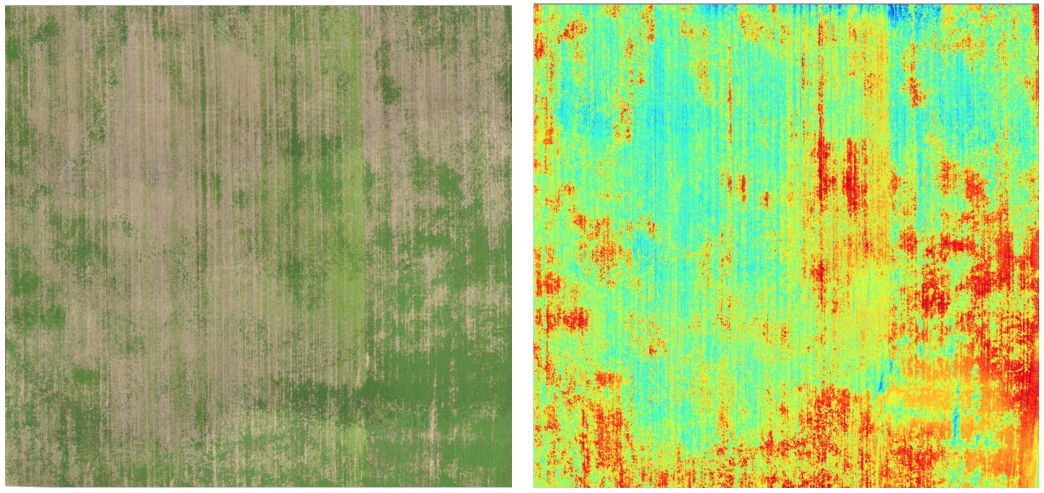
\includegraphics[width=1.0\textwidth]{images/ndvi.png}
    \caption{Left: RGB image of vegetation. Right: NDVI of the same vegetation, where hotter colors correspond to higher NDVI \cite{Abuleil}.}
    \label{ndvi_map}
\end{figure}

\subsection{Unmanned Aerial Systems}
Until recently, remote sensing has been performed by satellites, airplanes, balloons, and helicopters equipped with optical and near infrared sensors. However, there are several problems associated with these platforms. Firstly, due to the cost, these platforms are inaccessible to many farmers. Secondly, it is difficult to use these platforms on a regular basis. Ideally, farmers would collect data on their crops daily, analyze the data, and implement the necessary treatments by the next day. Finally, due to the high altitude from which the data is collected, the crops can be obscured by cloud cover or the data can suffer from low resolution. High resolution imagery is necessary for tasks such as weed detection. With weed detection, weeds must be located within an order of centimeters so that farmers can quickly find them in the fields \cite{Zhang2012}. In recent years, unmanned aerial systems have been purported as a solution to these problems.

\begin{figure}
    \centering
    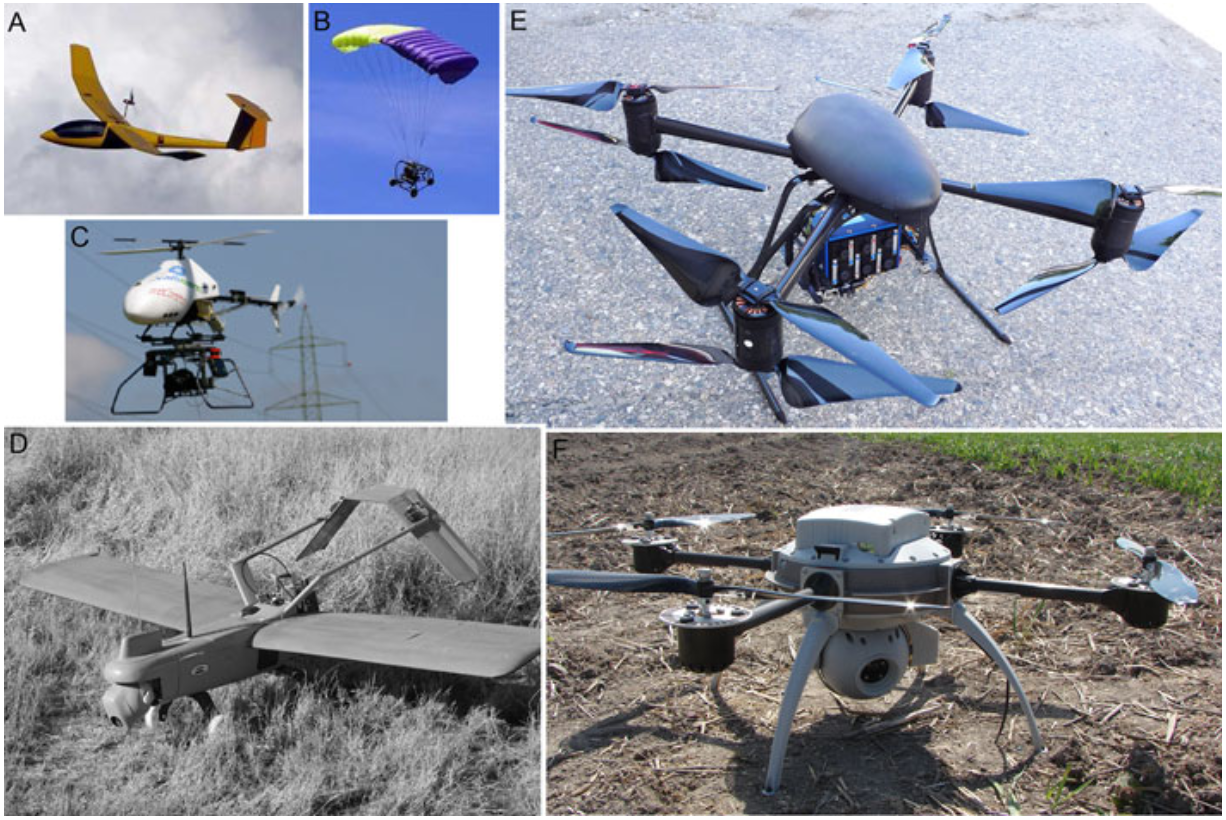
\includegraphics[width=1.0\textwidth]{images/uav.png}
    \caption{Examples of UAV. \textbf{a} powered glider, \textbf{b} powered parachute, \textbf{c} helicopter, \textbf{d} fixed wing aircraft, \textbf{e} Draganflyer X8 quadrocopter, \textbf{f} Aeryon Scout quadrocopter \cite{Zhang2012}}
    \label{UAV}
\end{figure}

Unmanned aerial vehicles (UAV) are small aircraft that can be piloted remotely usually taking the form of fixed wing airplanes, helicopters, and multicopters as seen in Figure \ref{UAV}. UAV have introduced a new paradigm of remote sensing referred to as low altitude remote sensing (LARS). These systems are characterized by their low operational costs, near real-time image acqusition, and high resolution imagery. However, UAV are not without their problems. Due to the relatively low altitude of the aircraft, many images must be captured to capture all of the field. With these images, it is necessary to perform image mosaicing, which adds a level of difficulty to the use of these systems. Additional issues arise from aviation regulations. In the United States, a Certificate of Authorization must be acquired and the UAV must always be in the view of the operator \cite{Zhang2012}. Despite these challenges, it seems that UAV are the best tools at our disposal for remote sensing.


\section{Machine Learning}
Machine learning is a set of methods that can automatically detect patterns in data, and use these patterns to predict future data or perform decision making \cite{Murphy}. With recent increases in data collection and computing performance, machine learning has found its way into nearly every part of modern technology. It is used in web searches, translation, image identification, translation, and consumer electronics \cite{Nature_DL}.

Within the realm of machine learning, there exist two main types: supervised learning and unsupervised learning. 

Supervised learning, the more common of the two, involves learning a mapping from an input $x$ to an output $y$, given a set of input-output pairs $D = \{(x_i, y_i)\}^N_{i=1}$. Where $D$ is the training set and $N$ is the number of examples in the training set \cite{Murphy}. Within supervised learning, problems are typically represented in two different ways: classification and regression. A classification problem has the goal of mapping an input into a discrete category. For example, given an image of a cat or dog $x$, predict the type of animal $y \in \{cat, dog\}$. A regression problem involves mapping an input to a continuous valued output \cite{Murphy}. For instance, given the height of a person $x$, predict the person's weight $y$, where $y \in \mathbb{R}$.

Unsupervised learning only considers the data $x$ without any targets $y$. The purpose behind this is to find any structure in the data to help perform the desired task. The typical tasks in unsupervised learning are clustering and dimensionality reduction. Clustering, as the name suggests, involves finding groups within the dataset $D$. For example, in e-commerce, users are often clustered into different groups based on their purchasing behavior. These learned clusters are then used for targeted advertising. Dimensionality reduction projects high dimensional data into lower dimensional space \cite{Murphy}. A simple example would be taking 3d data and reducing it into 2d space so that it can be easily displayed in a graph.

With any machine learning problem, it is important to define an objective function. This function will measure the error of the machine learning model's predictions from the ideal results. By doing this, it allows the model to update its parameters to reduce the error of the objective function. These parameters, or weights, can be seen as knobs that define the input-output function of the model. Most machine learning models update their parameters by finding the gradient vector of the objective function with respect to the model's parameters. Once the gradient vector is found, it is negated which makes it indicate the direction to change the parameters to decrease the error from the objective function. The negated gradient vector is then element-wise summed with the parameters of the model. This process describes a common optimization method in machine learning called Gradient Descent \cite{Nature_DL}. 

\subsection{Deep Learning}

Deep learning is a form of machine learning that has had many successes in recent years. This success is validated by its dominance in image and speech recognition competitions \cite{Nature_DL}. Older machine learning methods rely on domain experts to design feature extractors that transform raw data (such pixels of an image) into a representation that is easy for the algorithm to process. On the other hand, deep learning methods perform representation learning, which means that the algorithms will automatically discover good representations for the input data. Furthermore, deep learning methods are essentially a composition of many layers of representation learning modules. Each of these modules transform the input representation into a higher, more abstract level. With the composition of these transformations, complex functions can be learned.

\subsection{Feedforward Neural Networks}

\begin{figure}
    \centering
    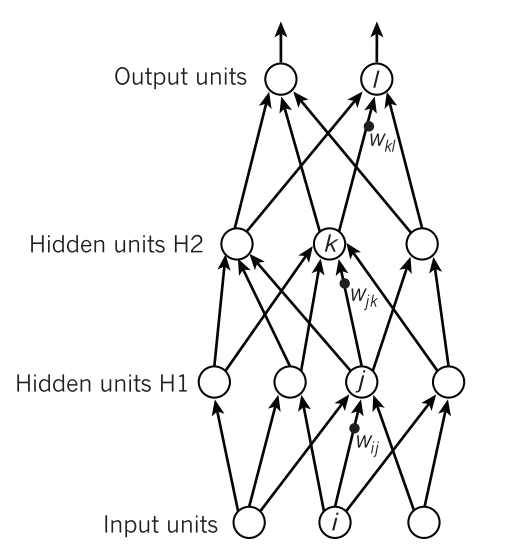
\includegraphics[width=0.5\textwidth]{images/mlp.png}
    \caption{A neural network that performs multiple levels of transformations \cite{Nature_DL}.}
    \label{mlp}
\end{figure}
Feedforward neural networks are the basis for various deep learning architectures. Neural networks, as they are concisely referred to, are composed of layers of units that compute a weighted sum of the inputs, which come from the previous layer, followed by a non-linear function. These layers are typically called dense layers or fully-connected layers. Currently, the most commonly used non-linear function is the rectified linear unit (ReLU), which takes the form of $f(z) = max(z, 0)$ \cite{Nature_DL}. Layers that are neither input nor output are considered to be hidden layers; these layers can take an arbitrary number nodes. An example neural network can be seen in Figure \ref{mlp}.

\subsection{Convolutional Neural Networks}
Convolutional neural networks (CNN) are inspired by the visual cortex and, as such, are optimal for processing images and other spatial data. These models did not become popular until the ImageNet competition of 2012. During this competition, a CNN was trained on millions of images of 1,000 different classes and achieved a result of half of the error of the best competing approaches. Since this success, it brought about a revolution in computer vision with CNNs being the dominant approach for recognition and detection tasks. Recently, CNNs have even approached human performance on some tasks \cite{Nature_DL}.

Convolutional neural networks are typically composed of three types of layers: convolution, pooling (sub-sampling), and dense. A convolutional layer involves sliding a fixed size filter, which can be represented as a matrix, across the input map while doing element-wise multiplication followed by a sum of the products. This operation works well with images because there is a high correlation between the local groups of values and because features in an image are invariant to location. The most common form of pooling is called max-pooling, which takes only the maximum value within a local patch of units to be in the output map. This has the effect of reducing the dimension of the representation and creating invariance to shifts and distortions \cite{Nature_DL}.

\begin{figure}
    \centering
    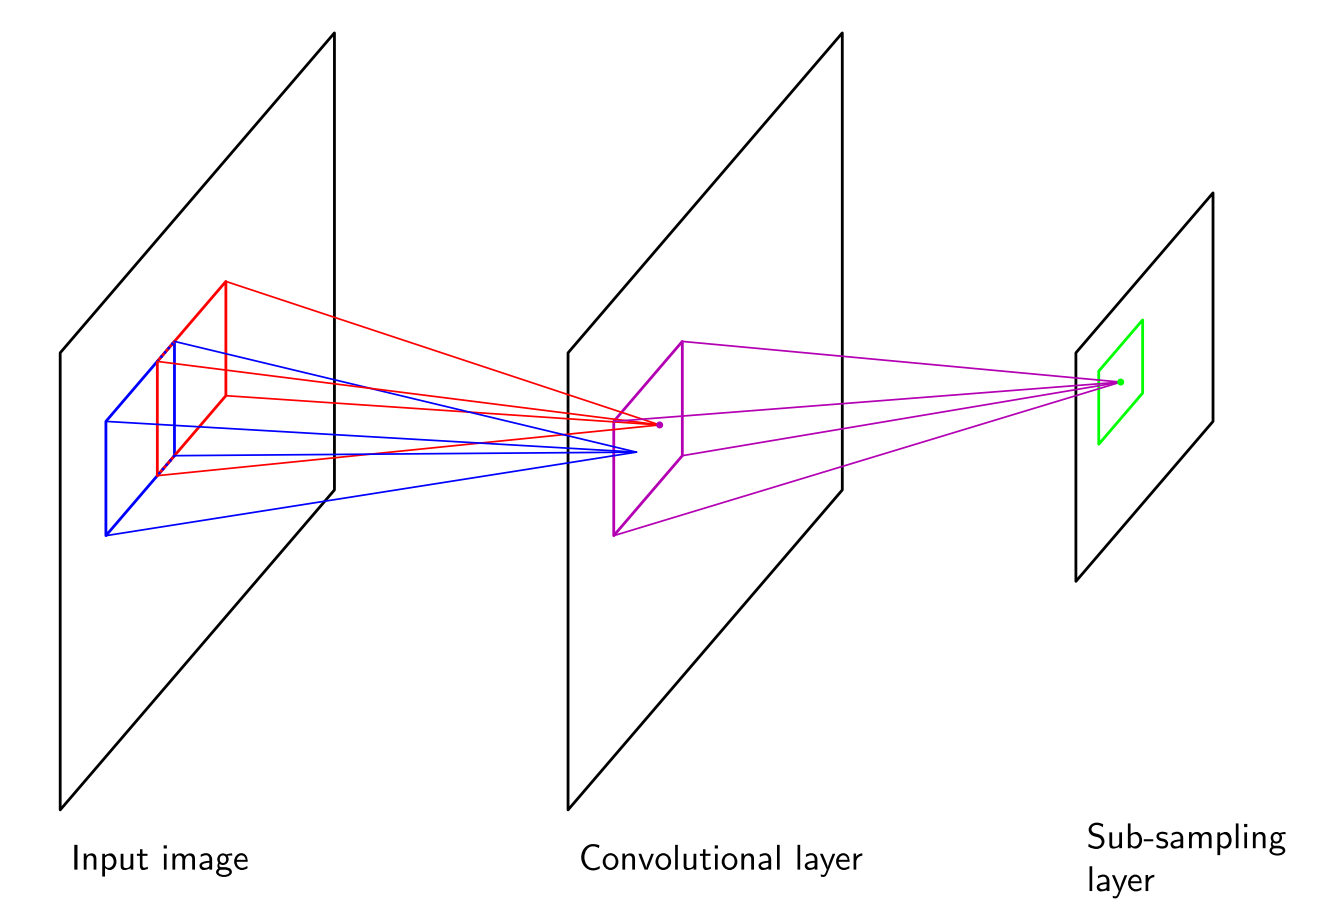
\includegraphics[width=0.8\textwidth]{images/conv.png}
    \caption{Convolutional layer followed by a pooling layer. \cite{Bishop2007}}
    \label{conv}
\end{figure}

Now that CNNs are the dominant method for vision related tasks, great effort is going into researching how to build the best performing model. There are many pieces of a CNN that can be adjusted. Firstly, the number of convolutional layers must be determined. Within the convolutional layers, the designer must consider the size of the filters, number of filters, and stride of the filters. Next, the number of max-pooling layers must be determined as well as the placement relative to the convolutional layers. At the end of the model, the number of dense layers as well as the number of units in each dense layer must be decided. Alternatively, some models do not even use dense layers at all. Besides configuring these existing layers, additional research is also going into new types of layers and new types of activation functions. In the following sections, we will explore several of the best CNN models.


\subsubsection{VGG}
\begin{figure}
    \centering
    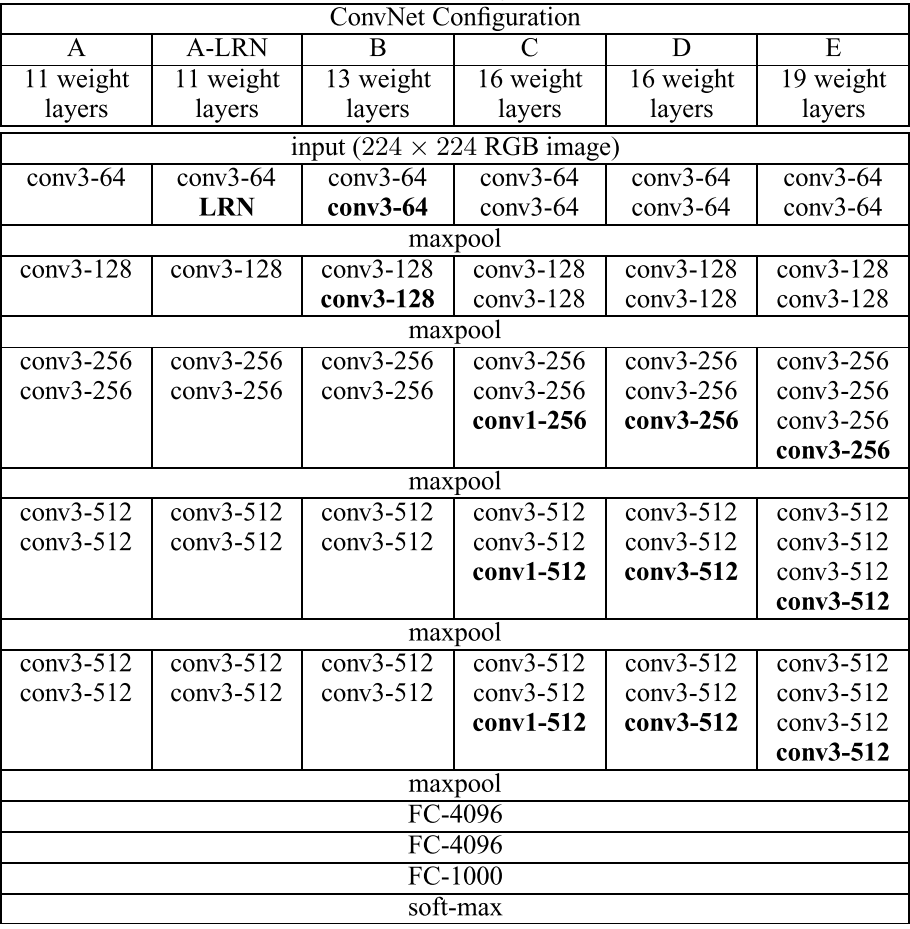
\includegraphics[width=0.8\textwidth]{images/vgg_arch.png}
    \caption{Architecture of VGG (typically D or E are selected). conv3-64 refers to a 3x3 convolution with 64 filters. FC-4096 refers to a dense layer with 4096 units \cite{vgg}.}
    \label{vgg}
\end{figure}
VGG is a CNN architecture that achieved first place in the ImageNet 2014 image localization task and second place in the image classification task. It is a fairly simple model as it consists almost entirely of 3x3 convolutional filters \cite{vgg}. It seems to be the most commonly chosen architecture for computer vision related tasks. This is likely due to its simplicity and availability in deep learning frameworks.

\subsubsection{ResNet}
\begin{figure}
    \centering
    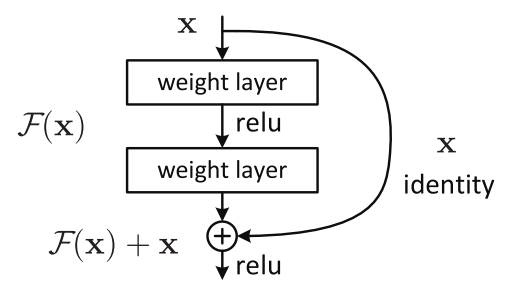
\includegraphics[width=0.65\textwidth]{images/residual.png}
    \caption{Residual block of ResNet. The weight layers will typically be convolutional layers. Many of these blocks are used throughout ResNet \cite{resnet}.}
    \label{residual}
\end{figure}
ResNet is a CNN from Microsoft research that achieved first place in the Imagenet competition in 2015. The main feature of this model is what is referred to as residual learning. Residual learning involves creating additional connections from one layer of the network to a deeper layer of the network bypassing several of the layers. The reason this is a useful technique is because a common problem with training deep neural networks is gradient explosion, which occurs when large gradients are multiplied by other larger gradients when optimizing a network. During this process, the gradients will become too large to be useful for training the network. Residual connections have the effect of allowing gradients to bypass several layers during training, which prevents the gradients from being multiplied as many times; therefore mitigating gradient explosion \cite{resnet}.

\subsubsection{DenseNet}
\begin{figure}
    \centering
    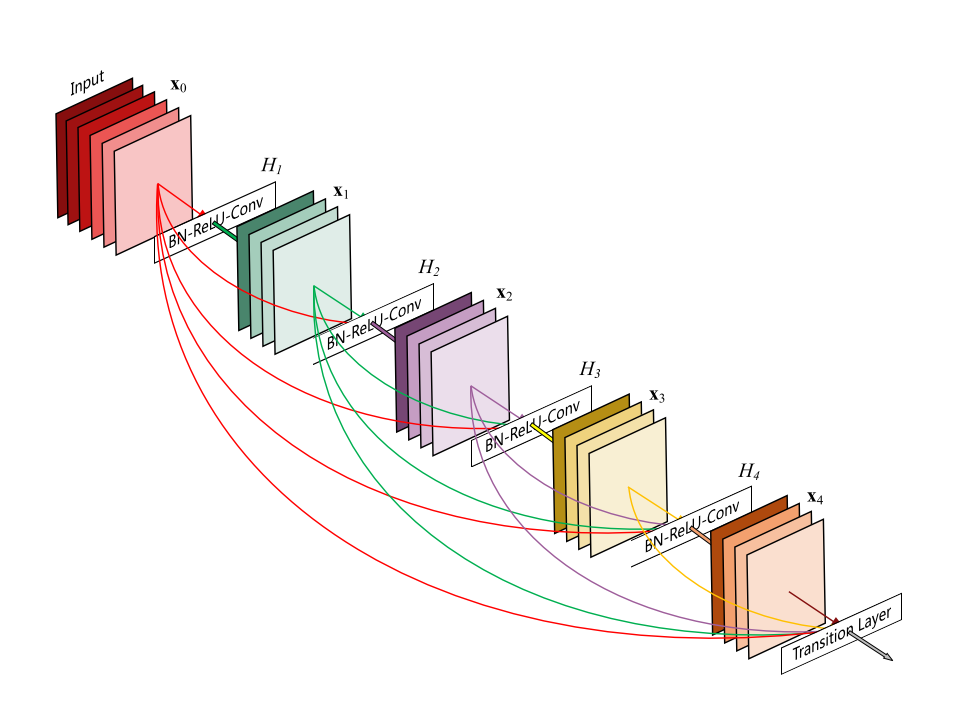
\includegraphics[width=0.65\textwidth]{images/denseblock.png}
    \caption{A dense block of 5 layers each with a growth rate of $k = 4$ \cite{densenet}.}
    \label{denseblock}
\end{figure}
DenseNet takes the idea of having residual connections from ResNet even further: all layers are directly connected with one another. Further, rather than summing the feature maps like in ResNet, DenseNet concatenates the maps instead. This high connectivity paired with concatenation allows maximum information flow in the network. One would think that the concatenation of the maps of each layer would lead to an excessive number of maps by the end of the network, but DenseNet achieves state-of-the-art results with fairly narrow layers ($k = 32$, where $k$ represents the number of output maps of each convolutional layer). In actuality, the dense connectivity requires fewer parameters than other CNNs because there is no need to re-learn redundant feature maps. One concern of having these connections is that all layers must have the same input and output size. Therefore, in order to allow downsizing of the feature maps, the authors consolidate these connected layers into a block that is referred to as a \emph{dense block}, as seen in Figure \ref{denseblock}. This allows the alternation between dense blocks and down-sampling layers to get high connectivity while allowing downsizing \cite{densenet}.


\subsubsection{Inception}
\begin{figure}
    \centering
    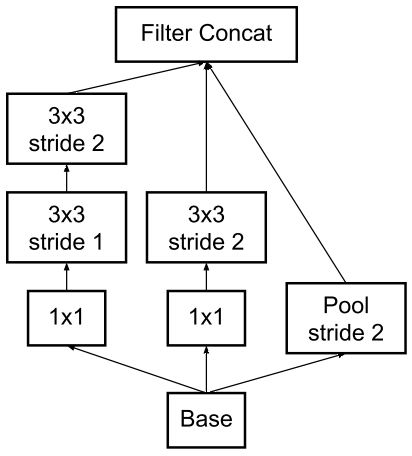
\includegraphics[width=0.50\textwidth]{images/inception.png}
    \caption{Inception block of Inception. It reduces the grid-size of the input map while increasing the number of filters \cite{inception}.}
    \label{inception_block}
\end{figure}
InceptionV3, which we will refer to as Inception from now on, is a CNN model that comes out of Google's research team. It has achieved the highest performance on Imagenet out of all of the models presented in this paper. Inception was designed to perform well under memory and computational constraints with the authors emphasizing a significant boost in performance compared to VGG. The main feature of this architecture is the Inception module. The Inception module is a section of the CNN that consists of concatenation of convolutions of various sizes. This has the effect of a reduction of the number of parameters in the network resulting in a reduction of parameters and, ultimately, a reduction in memory and computation \cite{inception}.


\subsubsection{Single Shot MultiBox Detector}
Single Shot MultiBox Detector (SSD) is a CNN that differs from the previous models in that it is used for detection tasks. This means that the CNN will not only determine the class of the object that appears in the image, but also determine the region in which the object appears. Furthermore, detectors can find multiple instances of a class or even different classes in the same image. SSD works by generating scores for the presence of each class in each default box, where boxes are a predetermined area of the image that an object can appear in. The network will also output adjustments to the box dimensions to create a better fit for the object. Experiments show that SSD is faster and more accurate than other state-of-the-art models on PASCAL VOC, a detection dataset. Impressively, the network is capable of running in real time: 59 frames per second for images of size 300x300 \cite{ssd}.

% Should we add RCNN or YOLO?

\subsubsection{FC-DenseNet}
\begin{figure}
    \centering
    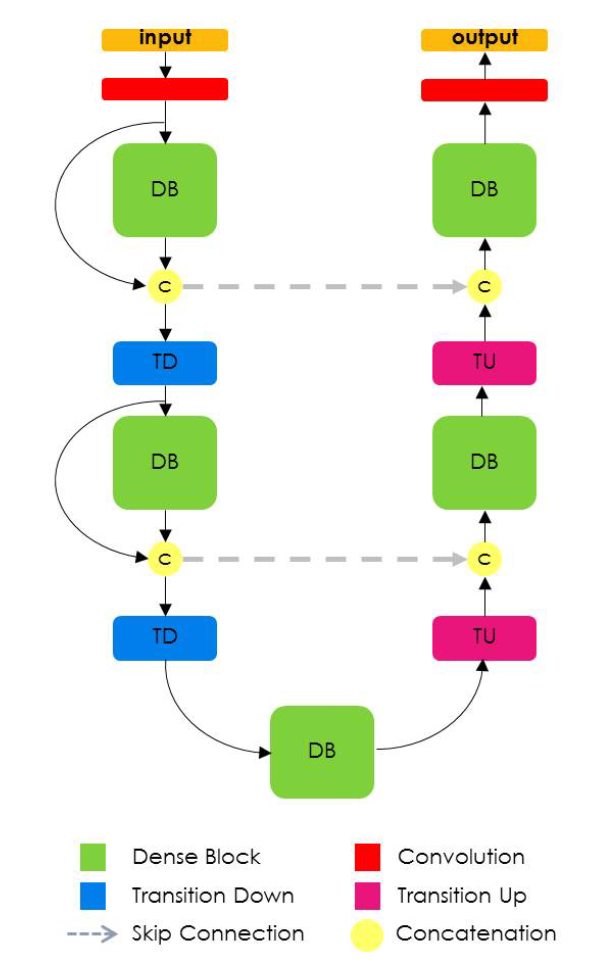
\includegraphics[width=0.40\textwidth]{images/fc-densenet.png}
    \caption{The architecture of FC-DenseNet \cite{fc-densenet}.}
    \label{fc-densenet}
\end{figure}
FC-DenseNet is a CNN that is used for semantic segmentation tasks, which involves determining a label for each pixel in the input image. As seen in Figure \ref{fc-densenet}, the architecture matches that of DenseNet by alternating dense blocks and transition-down blocks. The architecture differs by introducing a mirror of DenseNet where transition-down layers are replaced with transition-up layers, which are transposed convolution layers that upsample the previous feature maps. The most notable contribution of this architecture are the connections between the downsampling and upsampling paths. These connections help the upsampling path recover fine-grained information lost from the transition-down blocks \cite{fc-densenet}.

\subsection{Adam}
Adam is an algorithm for gradient-based optimization of functions. The algorithm draws inspiration from two previously created algorithms: RMSProp and Momentum. By combining these methods, Adam is able to bring a function to convergence more quickly than other optimizers in empirical results \cite{adam}. As a result of its high performance, Adam has become the most recommended optimizer in the deep learning community.
\subsection{Batch Normalization}
Batch Normalization (BN) is an additional layer in a neural network that performs normalization for each training batch. This method allows the use of higher learning rates, which leads to decreased training time. Furthermore, the authors' empirical results show increased accuracy in models using Batch Normalization \cite{batchnorm}.
\subsection{Dropout}
Dropout is a simple method used to prevent neural networks from overfitting. The technique involves randomly omitting nodes in a neural network during training time \cite{dropout}. The probability of node being omitted is controlled by a parameter $p$. Though counter-intuitive, this creates a better model because it forces all of the nodes of the network to contribute to predicting. In other words, the network cannot simply rely on a few strong nodes to make predictions as they may be randomly omitted.